% Final project proposal, ANLP -- ACL style.
%
% Build (Overleaf: pdfLaTeX + BibTeX, or just press Recompile):
%   pdflatex main && bibtex main && pdflatex main && pdflatex main
%
% Team: Claude's Plan. Rename the output PDF to ClaudesPlan-Proposal.pdf
%
% Requires, in the same directory: acl.sty, acl_natbib.bst, references.bib
%
\documentclass[11pt]{article}

% "preprint" = non-anonymous, with page numbers, no per-line numbering.
% Use "final" for a non-anonymous version without page numbers,
% or "review" for the anonymised, line-numbered version.
\usepackage[preprint]{acl}

\usepackage{times}
\usepackage{latexsym}
\usepackage[T1]{fontenc}
\usepackage[utf8]{inputenc}
\usepackage{microtype}
\usepackage{amsmath}
\usepackage{amssymb}
\usepackage{booktabs}
\usepackage{graphicx}

% acl.sty already loads natbib, geometry, caption and hyperref, and already
% sets \bibliographystyle{acl_natbib}. Do not load or set them again.

% The default title box (11 baselines) is too short for four authors plus
% roll numbers, team name, course, affiliation and the e-mail line.
\setlength\titlebox{6.4cm}

\title{Event-Anchored Representation Learning for\\
Neutral News Generation}

\author{
  \begin{tabular}{@{}cccc@{}}
    Chaitanya Thogata & Harshit Lalwani & Manas Agrawal & Raunak Seksaria \\
    {\normalfont (2023113018)} & {\normalfont (2023111028)} &
    {\normalfont (2023113023)} & {\normalfont (2023113019)} \\
  \end{tabular} \\[3pt]
  Team Name: Claude's Plan \\[1pt]
  {\normalfont Advanced NLP} \\[1pt]
  {\normalfont International Institute of Information Technology, Hyderabad} \\[1pt]
  {\normalfont\small\texttt{\{chaitanya.thogata, harshit.lalwani,}} \\
  {\normalfont\small\texttt{manas.agrawal, raunak.seksaria\}@research.iiit.ac.in}}
}

\begin{document}
\maketitle

\begin{abstract}
Recent work on neutral news generation suggests that shaping latent
representations may help mitigate framing bias. We propose to investigate
whether event identity can serve as the organizing principle of the
representation space. Our primary approach will use event-aware triplet
learning to bring representations of reports covering the same event closer
while separating carefully chosen contrasting reports, jointly with a neutral
text generation objective. Cross-report supervision will be used only during
training, while inference will operate on a single article. As an exploratory
extension, we also plan to study JEPA-style cross-report prediction, where the
representation of one same-event report is used to predict another. We will
evaluate whether these objectives improve neutrality, event retention, and
robustness to framing variation.
\end{abstract}

\section{Motivation}


News reports are not neutral observations of events. Different publishers may
emphasize different facts, use different language, omit details, or frame the
same occurrence through different editorial or ideological perspectives. This
makes neutralization difficult: a model must preserve the underlying event
while reducing reliance on source-specific presentation. Existing work
suggests that this problem is not purely about output wording. NeutraSum
directly shapes latent representations toward neutrality, while event-relation
graph methods show that explicitly modeling event information can improve
framing-bias mitigation and content preservation. These findings motivate us
to explore whether the shared information across differently framed reports
can provide a useful learning signal. Rather than treating any single source
as an authoritative account, multiple reports of the same occurrence can be
viewed as complementary views whose common content may better reflect the
information that should be preserved during neutralization.

\section{Related Work}

\textbf{NeuS: Neutral Multi-News Summarization for Mitigating Framing Bias} \citep{lee2022neus} introduced neutral summary generation from multiple news articles with different political leanings, motivated by the role of framing bias in political polarization. NeuS-Title uses the observation that titles provide a useful signal for framing bias and learns to neutralize news content from the title to the article. This establishes the multi-source neutral summarization setting that we build upon.

\textbf{Multi-document Summarization through Multi-document Event Relation Graph Reasoning in LLMs} \citep{lei2025multidoc} builds on the observation that events and event relations play an important role in media bias. It represents relationships within and across documents, including event coreference and event-level moral opinions, and incorporates this information into LLM-based summarization. The authors show improvements in both bias mitigation and content preservation. Our approach similarly treats event information as central to neutralization, but instead of explicitly constructing an event-relation graph, we use event identity to organize the model's latent representation.

\textbf{Tracing Partisan Bias to its Emotional Fingerprints: A Computational Approach to Mitigation} \citep{liu2025emotional} proposes that partisan bias is not merely an abstract stance, but materialises as quantifiable ``emotional fingerprints'' in news text. The authors use the Valence-Arousal-Dominance (VAD) framework to trace partisan stances to their linguistic roots and identify the affective strategies underlying partisan framing. This provides a complementary view of bias to representation-level approaches, by treating emotional language as an observable manifestation of partisan framing. We therefore use VAD as one of our evaluation dimensions to examine whether generated articles retain the emotional characteristics associated with partisan source articles.

\textbf{NeutraSum: A Language Model can help a Balanced Media Diet by Neutralizing News Summaries} \citep{neutrasum2025} addresses the observation that reports of the same event can differ substantially in language and focus depending on the political leaning of the outlet. It introduces two neutrality losses that adjust the semantic space of generated summaries by balancing their distances from polarized inputs and aligning them with expert-written summaries. Our approach similarly uses representation-level regularization, but uses cross-source event identity rather than direct neutrality constraints as the primary organizing signal.

\textbf{We Can Detect Your Bias: Predicting the Political Ideology of News Articles} \citep{baly2020detect} studies whether political ideology can be predicted from news articles while preventing models from simply learning the identity of the source. The authors use both adversarial media adaptation and a specially designed triplet loss, with examples from different media used to encourage representations that capture ideology rather than source identity. We adapt this underlying idea to a different objective: rather than preserving ideology while removing publisher information, we aim to bring reports of the same event together while separating reports of different events from the same publisher.

Finally, our exploratory JEPA-style extension is inspired by \textbf{Self-Supervised Learning From Images With a Joint-Embedding Predictive Architecture} \citep{assran2023ijepa}. I-JEPA learns by predicting the representation of one view from another rather than reconstructing the input itself. We propose to treat reports from different outlets covering the same event as such cross-source views, with the expectation that their shared representation will capture information about the underlying event while being less dependent on source-specific variation.

\section{Contribution}

Our work proposes to use event identity as a central supervisory signal for neutral news generation. We use relationships between different reports of the same event to shape encoder representations, with triplet objectives based on either publisher or ideological variation. Cross-report information is used during training, while the resulting model is intended to neutralize a single article at inference time.

Our approach offers three complementary contributions:

\begin{itemize}
\item Representation learning: instead of explicitly constructing event-relation graphs or directly constraining representations toward political neutrality, we learn event-focused structure from cross-report relationships.
\item Content-preserving evaluation: a summary may appear neutral simply by deleting disagreement or framed information. We therefore evaluate event-information retention separately from neutrality, explicitly measuring whether reduced bias comes at the cost of losing important content.
\item JEPA-style prediction: we explore predicting the representation of one same-event report from another, allowing shared event information to emerge without explicitly defining publisher- or ideology-based contrasts.
\end{itemize}

\section{Methodology}

\subsection{Event-Aware Triplet Learning}

We plan to use triplet learning to encourage the encoder to organize article representations around the underlying event. The final encoder hidden states of each article will be pooled into an article-level embedding. Given an anchor \(a\), positive \(p\), and negative \(n\),

$$ \mathcal{L}_{\text{triplet}} = \max\big(D(a,p)-D(a,n)+\alpha,\;0\big), $$

where \(D(\cdot,\cdot)\) is Euclidean distance and \(\alpha\) is a margin.

\subsection{Triplet Construction}

We will test two variants: publisher-based and ideology-based triplets. In both cases, the positive shares the anchor event while the negative changes the event but preserves the selected contrasting factor. Figure~\ref{fig:triplets} illustrates both variants.

\begin{figure}[t]
\centering
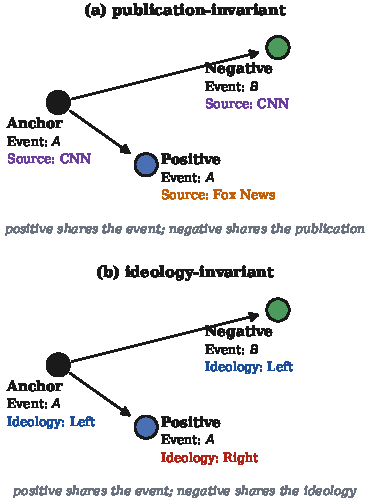
\includegraphics[width=0.85\linewidth]{triplets}
\caption{The two triplet variants under consideration: (a) publisher-based, where the positive shares the event with the anchor and the negative shares the publisher; (b) ideology-based, where the positive shares the event and the negative shares the anchor's ideology label instead.}
\label{fig:triplets}
\end{figure}

\subsection{Joint Objective and Architecture}

The model will be jointly optimized using

$$ \mathcal{L} = \mathcal{L}_{\text{LED}} + \lambda\mathcal{L}_{\text{triplet}}, $$

where \(\mathcal{L}_{\text{LED}}\) is the neutral text generation loss.

We plan to use LED-base-16384 \citep{beltagy2020longformer}, potentially scaling to LED-large. LED retains a BART-style encoder-decoder architecture while supporting substantially longer inputs through sparse attention. Encoder states will be pooled for triplet learning and passed to the decoder for neutral generation. At inference time, only a single article will be required.

\begin{figure}[t]
\centering
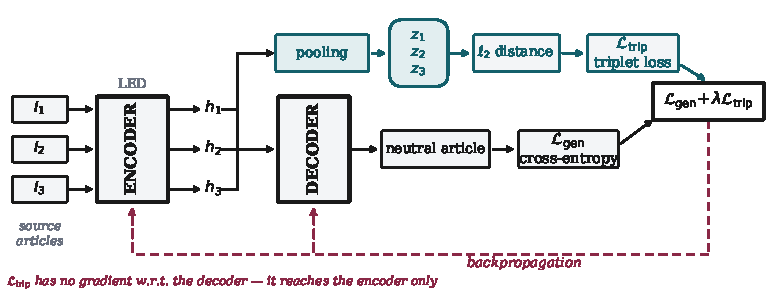
\includegraphics[width=\linewidth]{architecture}
\caption{Model architecture: the shared encoder feeds both the decoder, under $\mathcal{L}_{\text{LED}}$, and a pooled triplet loss $\mathcal{L}_{\text{triplet}}$ over the encoder representations. The triplet loss has no gradient with respect to the decoder; it reaches the encoder only.}
\label{fig:architecture}
\end{figure}

\subsection{Exploratory JEPA Pretraining}

We also plan to explore JEPA-style cross-report prediction, where one same-event report is used to predict the latent representation of another. This requires only same-event pairs and may encourage the representation to retain information shared across reports.

\subsection{Datasets}

\begin{table}[t]
\centering\small
\begin{tabular}{@{}lccc@{}}
\toprule
\textbf{Dataset} & \textbf{Event} & \textbf{Ideology} & \textbf{Publisher} \\
\midrule
NeuS / AllSides & \checkmark & \checkmark & \checkmark \\
WCEP-10 & \checkmark & $\times$ & $\times$ \\
Article-Bias-Prediction & $\times$ & \checkmark & \checkmark \\
\bottomrule
\end{tabular}
\caption{Dataset sizes: NeuS / AllSides, 3{,}095 stories / 9{,}282 articles; WCEP-10, 10{,}200 event clusters; Article-Bias-Prediction, 37{,}554 articles / 491 outlets.}
\label{tab:datasets}
\end{table}

NeuS/AllSides will be the main supervised dataset, WCEP-10 will support JEPA pretraining, and Article-Bias-Prediction will provide additional negatives and unseen-publisher evaluation. Neutral generation targets will either come from a suitable neutral-reference dataset or be generated synthetically using LLM inference.

\section{Evaluation Plan}

\paragraph{Ablations.} We use two models, one a control LED model without our triplet loss and another model trained with our triplet loss, and compare all metrics in both cases to verify causality in any significant results.

\paragraph{Information Retention:}

1. Question-Answer Coverage: We create question-answer pairs based on the original articles, and then evaluate whether the newly generated articles contain the answers to these questions.

a. We do this on our own evaluation dataset using FeQA \citep{durmus2020feqa} (possibly expensive in time and compute).

b. We can evaluate our model on the existing DiverseSum dataset of news articles. However, we cannot analyze the model's bias in QA coverage across political articles of different ideologies (i.e., considering source left and right articles, it may ignore facts mentioned in a right article but not in a left article). To evaluate this, we need a dataset of articles labelled with their political ideologies. Also, it may be unfair to perform different evaluations on different datasets. Considering the lack of labeling for political ideologies, we cannot run certain other evaluations on DiverseSum.
\paragraph{Tonality:} We use VAD (Valence, Arousal, Dominance) to analyze the tonality of the article.
\paragraph{Publisher Leakage:} We use existing publisher classifiers for news articles and run them on the source articles and output articles. We expect the F1 metric to decrease, ideally to the same as a random baseline.
\paragraph{Ideological Neutrality:} We use existing political ideology classifiers for news articles and expect them to report low confidence on all ideologies or high confidence on centrist ideology (depending on whether we take centrist as a proxy for neutral or not).

\section{Impact and Future Work}

This work can help quantify how strongly publisher identity is encoded in news representations and whether reducing such information improves neutrality without sacrificing event content. It may also provide insight into how separable event, publisher, and ideological information are within the learned representation space. The neutralized outputs could potentially be used to create less source-dependent corpora for training or evaluating downstream NLP models. If JEPA-style cross-report learning proves effective, it could enable scalable pretraining on large collections of same-event articles without requiring publisher labels, ideology annotations, or neutral targets, while also demonstrating the usefulness of predictive joint-embedding objectives for NLP.

\section{Limitations}

\begin{itemize}
\item Our model cannot identify complex problems such as flawed logic.
\item There is no objective measure of neutrality, nor could we find relevant data that could be labeled as neutral to a significant extent.
\item The political ideology classifiers we use are vulnerable to syntactic-level gaming (i.e., simply learning the writing style of different news outlets and using the fact that they are often biased towards the same ideologies).
\item Our generated articles will very likely lose some information mentioned in one or more source articles. Hiding any significant information is itself a form of bias. While we do try to measure coverage, it would be difficult to achieve good coverage with such small models.
\end{itemize}

\section{Ethical considerations}

The primary ethical concern of this work is that a system intended to generate politically neutral news summaries may itself introduce, preserve, or conceal political bias. In particular, removing publisher-specific information does not necessarily guarantee neutrality, and the model may omit information from one or more sources or generate unsupported information. Such outputs could influence readers' understanding of political events if used without human oversight. We therefore treat neutrality and information retention as separate evaluation objectives and explicitly report the limitations of the evaluation metrics and political ideology classifiers used. The system is intended as a research prototype for studying neutral multi-source summarization rather than as a replacement for journalistic judgment or as a source of authoritative political information.

\section{Timeline}

\begin{table}[h]
\centering\small
\begin{tabular}{@{}ll@{}}
\toprule
\textbf{Weeks} & \textbf{Milestone} \\
\midrule
1--2   & Data pipeline and evaluation setup \\
3--4   & LED-base baseline \\
5--6   & Triplet loss + initial results \\
Mid-eval & Baseline results + first triplet \\
       & result (if completed) \\
7--8   & Probing and ablations \\
9--10  & Full evaluation and generalization \\
11--12 & Final experiments, analysis, and report \\
\bottomrule
\end{tabular}
\caption{Planned schedule.}
\label{tab:timeline}
\end{table}

{\small\textit{Note: JEPA-style cross-report pretraining will be treated as an optional extension and explored only if time and compute permit.}}

\bibliography{references}

\end{document}
